% Options for packages loaded elsewhere
\PassOptionsToPackage{unicode}{hyperref}
\PassOptionsToPackage{hyphens}{url}
%
\documentclass[
]{article}
\usepackage{amsmath,amssymb}
\usepackage{lmodern}
\usepackage{ifxetex,ifluatex}
\ifnum 0\ifxetex 1\fi\ifluatex 1\fi=0 % if pdftex
  \usepackage[T1]{fontenc}
  \usepackage[utf8]{inputenc}
  \usepackage{textcomp} % provide euro and other symbols
\else % if luatex or xetex
  \usepackage{unicode-math}
  \defaultfontfeatures{Scale=MatchLowercase}
  \defaultfontfeatures[\rmfamily]{Ligatures=TeX,Scale=1}
\fi
% Use upquote if available, for straight quotes in verbatim environments
\IfFileExists{upquote.sty}{\usepackage{upquote}}{}
\IfFileExists{microtype.sty}{% use microtype if available
  \usepackage[]{microtype}
  \UseMicrotypeSet[protrusion]{basicmath} % disable protrusion for tt fonts
}{}
\makeatletter
\@ifundefined{KOMAClassName}{% if non-KOMA class
  \IfFileExists{parskip.sty}{%
    \usepackage{parskip}
  }{% else
    \setlength{\parindent}{0pt}
    \setlength{\parskip}{6pt plus 2pt minus 1pt}}
}{% if KOMA class
  \KOMAoptions{parskip=half}}
\makeatother
\usepackage{xcolor}
\IfFileExists{xurl.sty}{\usepackage{xurl}}{} % add URL line breaks if available
\IfFileExists{bookmark.sty}{\usepackage{bookmark}}{\usepackage{hyperref}}
\hypersetup{
  pdftitle={Econometria 2},
  pdfauthor={Miguel Sallum},
  hidelinks,
  pdfcreator={LaTeX via pandoc}}
\urlstyle{same} % disable monospaced font for URLs
\usepackage[margin=1in]{geometry}
\usepackage{color}
\usepackage{fancyvrb}
\newcommand{\VerbBar}{|}
\newcommand{\VERB}{\Verb[commandchars=\\\{\}]}
\DefineVerbatimEnvironment{Highlighting}{Verbatim}{commandchars=\\\{\}}
% Add ',fontsize=\small' for more characters per line
\usepackage{framed}
\definecolor{shadecolor}{RGB}{248,248,248}
\newenvironment{Shaded}{\begin{snugshade}}{\end{snugshade}}
\newcommand{\AlertTok}[1]{\textcolor[rgb]{0.94,0.16,0.16}{#1}}
\newcommand{\AnnotationTok}[1]{\textcolor[rgb]{0.56,0.35,0.01}{\textbf{\textit{#1}}}}
\newcommand{\AttributeTok}[1]{\textcolor[rgb]{0.77,0.63,0.00}{#1}}
\newcommand{\BaseNTok}[1]{\textcolor[rgb]{0.00,0.00,0.81}{#1}}
\newcommand{\BuiltInTok}[1]{#1}
\newcommand{\CharTok}[1]{\textcolor[rgb]{0.31,0.60,0.02}{#1}}
\newcommand{\CommentTok}[1]{\textcolor[rgb]{0.56,0.35,0.01}{\textit{#1}}}
\newcommand{\CommentVarTok}[1]{\textcolor[rgb]{0.56,0.35,0.01}{\textbf{\textit{#1}}}}
\newcommand{\ConstantTok}[1]{\textcolor[rgb]{0.00,0.00,0.00}{#1}}
\newcommand{\ControlFlowTok}[1]{\textcolor[rgb]{0.13,0.29,0.53}{\textbf{#1}}}
\newcommand{\DataTypeTok}[1]{\textcolor[rgb]{0.13,0.29,0.53}{#1}}
\newcommand{\DecValTok}[1]{\textcolor[rgb]{0.00,0.00,0.81}{#1}}
\newcommand{\DocumentationTok}[1]{\textcolor[rgb]{0.56,0.35,0.01}{\textbf{\textit{#1}}}}
\newcommand{\ErrorTok}[1]{\textcolor[rgb]{0.64,0.00,0.00}{\textbf{#1}}}
\newcommand{\ExtensionTok}[1]{#1}
\newcommand{\FloatTok}[1]{\textcolor[rgb]{0.00,0.00,0.81}{#1}}
\newcommand{\FunctionTok}[1]{\textcolor[rgb]{0.00,0.00,0.00}{#1}}
\newcommand{\ImportTok}[1]{#1}
\newcommand{\InformationTok}[1]{\textcolor[rgb]{0.56,0.35,0.01}{\textbf{\textit{#1}}}}
\newcommand{\KeywordTok}[1]{\textcolor[rgb]{0.13,0.29,0.53}{\textbf{#1}}}
\newcommand{\NormalTok}[1]{#1}
\newcommand{\OperatorTok}[1]{\textcolor[rgb]{0.81,0.36,0.00}{\textbf{#1}}}
\newcommand{\OtherTok}[1]{\textcolor[rgb]{0.56,0.35,0.01}{#1}}
\newcommand{\PreprocessorTok}[1]{\textcolor[rgb]{0.56,0.35,0.01}{\textit{#1}}}
\newcommand{\RegionMarkerTok}[1]{#1}
\newcommand{\SpecialCharTok}[1]{\textcolor[rgb]{0.00,0.00,0.00}{#1}}
\newcommand{\SpecialStringTok}[1]{\textcolor[rgb]{0.31,0.60,0.02}{#1}}
\newcommand{\StringTok}[1]{\textcolor[rgb]{0.31,0.60,0.02}{#1}}
\newcommand{\VariableTok}[1]{\textcolor[rgb]{0.00,0.00,0.00}{#1}}
\newcommand{\VerbatimStringTok}[1]{\textcolor[rgb]{0.31,0.60,0.02}{#1}}
\newcommand{\WarningTok}[1]{\textcolor[rgb]{0.56,0.35,0.01}{\textbf{\textit{#1}}}}
\usepackage{graphicx}
\makeatletter
\def\maxwidth{\ifdim\Gin@nat@width>\linewidth\linewidth\else\Gin@nat@width\fi}
\def\maxheight{\ifdim\Gin@nat@height>\textheight\textheight\else\Gin@nat@height\fi}
\makeatother
% Scale images if necessary, so that they will not overflow the page
% margins by default, and it is still possible to overwrite the defaults
% using explicit options in \includegraphics[width, height, ...]{}
\setkeys{Gin}{width=\maxwidth,height=\maxheight,keepaspectratio}
% Set default figure placement to htbp
\makeatletter
\def\fps@figure{htbp}
\makeatother
\setlength{\emergencystretch}{3em} % prevent overfull lines
\providecommand{\tightlist}{%
  \setlength{\itemsep}{0pt}\setlength{\parskip}{0pt}}
\setcounter{secnumdepth}{-\maxdimen} % remove section numbering
\usepackage[brazilian]{babel}
\usepackage[utf8]{inputenc}
\ifluatex
  \usepackage{selnolig}  % disable illegal ligatures
\fi

\title{Econometria 2}
\author{Miguel Sallum}
\date{23/06/2021}

\begin{document}
\maketitle

\hypertarget{regressuxe3o-linear-e-estimauxe7uxe3o}{%
\subsection{Regressão Linear e
Estimação}\label{regressuxe3o-linear-e-estimauxe7uxe3o}}

A regressão linear é um modelo de relação entre variáveis, e pode ser
chamado também de função de esperança condicional. Ela é
tradicionalmente estimada com método dos mínimos quadrados ordinários,
mas é equivalente por método dos momentos e (se não me engano) por
máxima verossimilhança.

Caso tenhamos somente um regressor, estamos estimando a esperança
condicional da forma \[
E[Y|X]\ =\ \beta_0\ +\ \beta_1X
\] Tradicionalmente, no entanto, representamos o modelo como \[
Y\ =\ \beta_0\ +\ \beta_1X +\mu
\] Onde \(\mu\) são os fatores não observados. Para estimarmos as
regressões, são necessárias algumas hipóteses: 1. É importante lembrar
que a regressão \emph{não é} um modelo causal. Para ser causal, são
necessárias algumas hipóteses a mais. Sendo flexível com notação, em
geral nosso interesse é estimar o modelo causal \[
E[Y|do(X)]\ =\ \beta_0\ +\ \beta_1X
\] Queremos encontrar então o valor adequado de \(\beta_1\), que seria o
efeito médio de X sobre Y. para isso, precisamos da hipótese
\textbf{(não-observável)} 4. \(Corr(X,\mu )=0\)

\hypertarget{estimauxe7uxe3o-matricial}{%
\subsubsection{Estimação matricial}\label{estimauxe7uxe3o-matricial}}

\hypertarget{muxe9todos-do-r-e-bibliotecas}{%
\subsubsection{Métodos do R e
Bibliotecas}\label{muxe9todos-do-r-e-bibliotecas}}

\hypertarget{potencial-outcomes}{%
\subsection{Potencial Outcomes}\label{potencial-outcomes}}

Potencial Outcomes é uma forma de pensar sobre causalidade usando de
contrafactuais. A ideia é que teríamos a informação do resultado de cada
indivíduo para cada nível de intervenção de X. Os exemplos do tema em
geral são binários, \textbf{mas o método não se restringe a isso}.

\begin{Shaded}
\begin{Highlighting}[]
\FunctionTok{summary}\NormalTok{(cars)}
\end{Highlighting}
\end{Shaded}

\begin{verbatim}
##      speed           dist       
##  Min.   : 4.0   Min.   :  2.00  
##  1st Qu.:12.0   1st Qu.: 26.00  
##  Median :15.0   Median : 36.00  
##  Mean   :15.4   Mean   : 42.98  
##  3rd Qu.:19.0   3rd Qu.: 56.00  
##  Max.   :25.0   Max.   :120.00
\end{verbatim}

\hypertarget{matching-e-estratificauxe7uxe3o}{%
\subsection{Matching e
Estratificação}\label{matching-e-estratificauxe7uxe3o}}

You can also embed plots, for example:

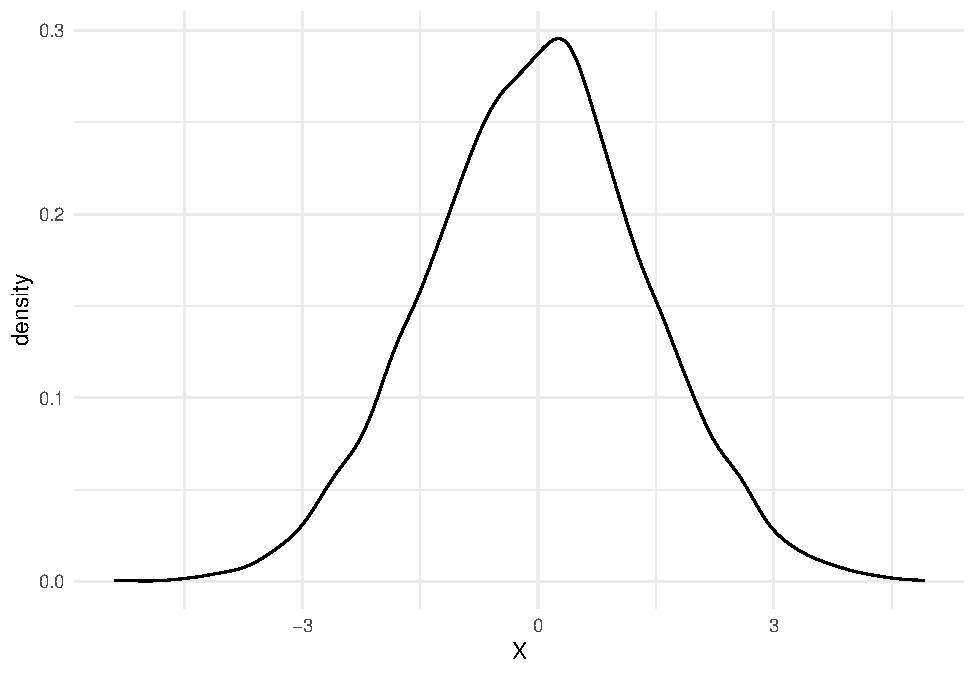
\includegraphics{Resumo_semestre_files/figure-latex/pressure-1.pdf}

Note that the \texttt{echo\ =\ FALSE} parameter was added to the code
chunk to prevent printing of the R code that generated the plot.

\hypertarget{regression-discontinuity-design}{%
\subsection{Regression Discontinuity
Design}\label{regression-discontinuity-design}}

\hypertarget{variuxe1vel-instrumental}{%
\subsection{Variável Instrumental}\label{variuxe1vel-instrumental}}

\hypertarget{panel-data}{%
\subsection{Panel Data}\label{panel-data}}

\hypertarget{diferenuxe7as-em-diferenuxe7as}{%
\subsection{Diferenças-em-Diferenças}\label{diferenuxe7as-em-diferenuxe7as}}

\hypertarget{event-study-two-way-fixed-effects-e-generalizauxe7uxe3o-de-did}{%
\subsection{Event Study, Two-Way Fixed Effects e Generalização de
DiD}\label{event-study-two-way-fixed-effects-e-generalizauxe7uxe3o-de-did}}

\end{document}
